% In this segment, enter the desired data to be shown at the title page
\newcommand{\Authors}{Max Perraudin}
\newcommand{\Title}{Template}
\newcommand{\SubTitle}{\Project}
\newcommand{\Projectdescription}{Description.}
\newcommand{\Project}{Project name}
\newcommand{\university}{University or school}
\newcommand{\Date}{\today}
\newcommand{\company}{Company}
\newcommand{\Tuteur}{\small Company tutor : \large tutor1 \\ \small School tutor : \large tutor2}

% don't forget to change the figures below
%------------------------------------------------------------------------------
\begin{titlepage}
\thispagestyle{empty}
\myfont

\begin{figure} [H]
    \vspace{-2cm}
    \centering
    \begin{minipage}[t]{.45\linewidth}
        % Adjust placement with this \vspace{-2.6cm} or this \hspace*{-0.5cm}
        \raggedright
        \includegraphics[width=1.\linewidth]{logo1.png}
    \end{minipage}%
    \begin{minipage}[t]{.45\linewidth}
        % Adjust placement with this \vspace{-2.6cm} or this \hspace*{0.5cm}
        \raggedleft
        \includegraphics[width =1.\textwidth]{logo2.png} 
    \end{minipage}
\end{figure}



% Adds background picture. Delete code if no background picture is wanted.
\begin{tikzpicture}[overlay, remember picture]
\node[anchor=south west, 
      xshift=-0.2cm, 
      yshift=-1.5cm] 
     at (current page.south west)
     {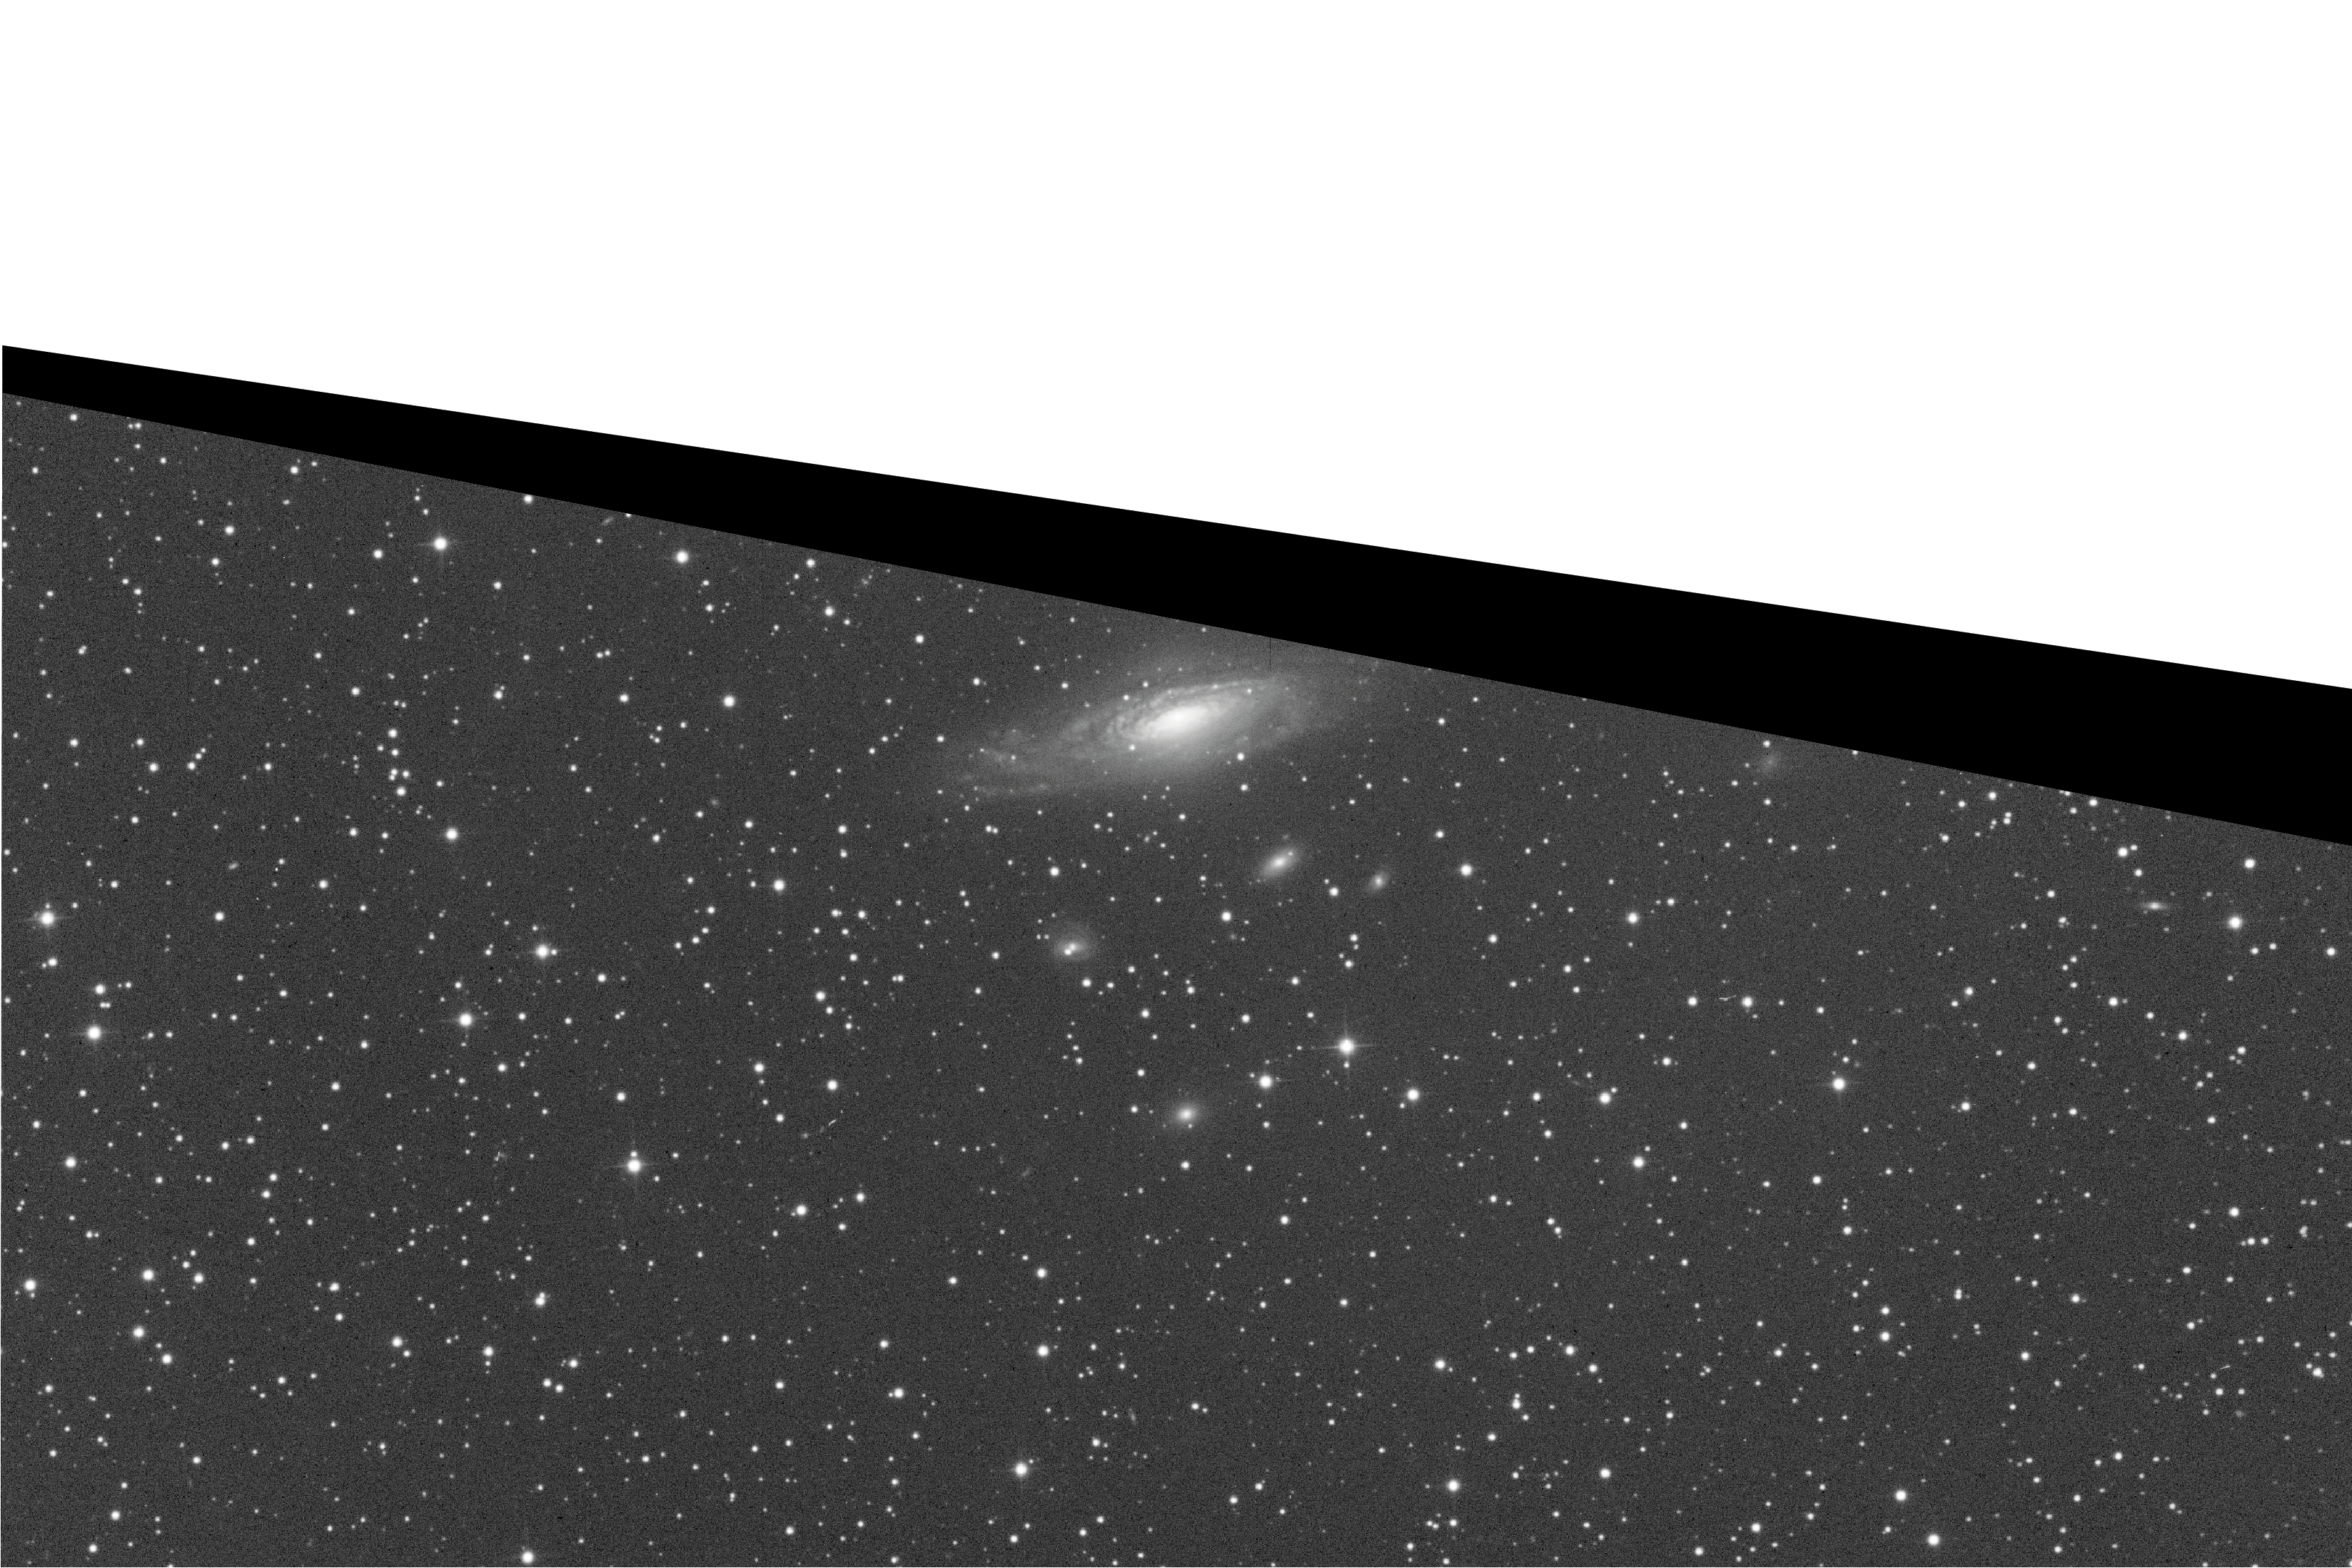
\includegraphics[width=22cm]{Figures/background.png}}; 
\end{tikzpicture}


\vspace{1 cm}
\par
\noindent
\Huge
\textbf{\Title}
\vspace{0.2cm}
\LARGE
\par
\noindent
\SubTitle\\
\rule[0.3cm]{\linewidth}{2pt}
\Large


\noindent
\small
\textit{\Projectdescription}

\vspace{0.5cm}
\noindent
\large
\Authors
\par \noindent
\raggedleft
\Tuteur
\vspace{0.5 cm}
\small
%\par \noindent
%\university
%\par \noindent
%\company
\par \noindent
\Date

\end{titlepage}